\documentclass[10pt,a4paper]{article}
\usepackage{amsmath}
\usepackage{graphicx}
\usepackage{amsfonts}
\usepackage{float} % useful for H in figures
\usepackage{hyperref} % useful for the \path command
\usepackage[font={footnotesize}]{caption}
\graphicspath{{../figures/}}

\usepackage{fontspec}
% \setmonofont{DejaVu Sans Mono}[Scale=0.8]
\setmonofont{Consolas}[Scale=0.85]




\begin{document}


\section*{SciML 2022 Exam}

This is the exam solution for Christian Michelsen in the Ph.D. course SciML 2022 at DTU.
All data is available at: \url{https://github.com/ChristianMichelsen/SciML2022-exam}.

\vspace{1cm}

\noindent The exam is based on the following problems:
\begin{enumerate}
    \item Solve a damped harmonic oscillator with known parameters and generate data from the ODE solution
    \item Fit the data with a non-damped harmonic oscillator using a neural network to model the missing dynamics
    \item Symbolically recover the missing terms of the ODE (i.e. retrieve the original damped ODE)
    \item Fit the data from 1) using Turing (but with unknown parameters), and quantify the uncertainties
\end{enumerate}

\clearpage
\section*{1: Damped Harmonic Oscillator}

The damped harmonic oscillator (DHO) is, as the name suggests, a damped version of the classical harmonic oscillator (HO):
\begin{equation}
    m \ddot{x} + b\dot{x} + kx = 0.
    \label{eq:DHO}
\end{equation}
The dampening is determined by the damping parameter $b$, the mass is $m$, and the spring constant is $k$.
Here $\dot{x}$ refers to the first derivative of $x$ with respect to time $t$, and $\ddot{x}$ refers to the second derivative of $x$.
As such, the DHO is an differential equation governed by Newton's second law (the first term),
Hook's law (the last term) and the friction term (the second term).

Without loss of generality, I set $m=1$ and use dimensionless variables.
Equation \eqref{eq:DHO} can then be transformed to the following system:
\begin{equation}
    \begin{split}
        \dot{x} &= v \\
        \dot{v} &= -kx - bv.
    \end{split}
    \label{eq:DHO_2D}
\end{equation}

I solve \eqref{eq:DHO_2D} using \texttt{DifferentialEquations.jl} in Julia with the following parameters:
\begin{equation}
    \begin{split}
        b &= 0.1 \\
        k &= 0.1 \\
        x_0 &= 1.0 \\
        v_0 &= 1.0 \\
        t &\in [0, 40],
    \end{split}
\end{equation}
where $x_0$ and $v_0$ are the initial conditions for $x$ and $v$.
The solution to \eqref{eq:DHO} can be seen in Figure \ref{fig:DHO} as the solid, blue line.

\begin{figure}[H]
    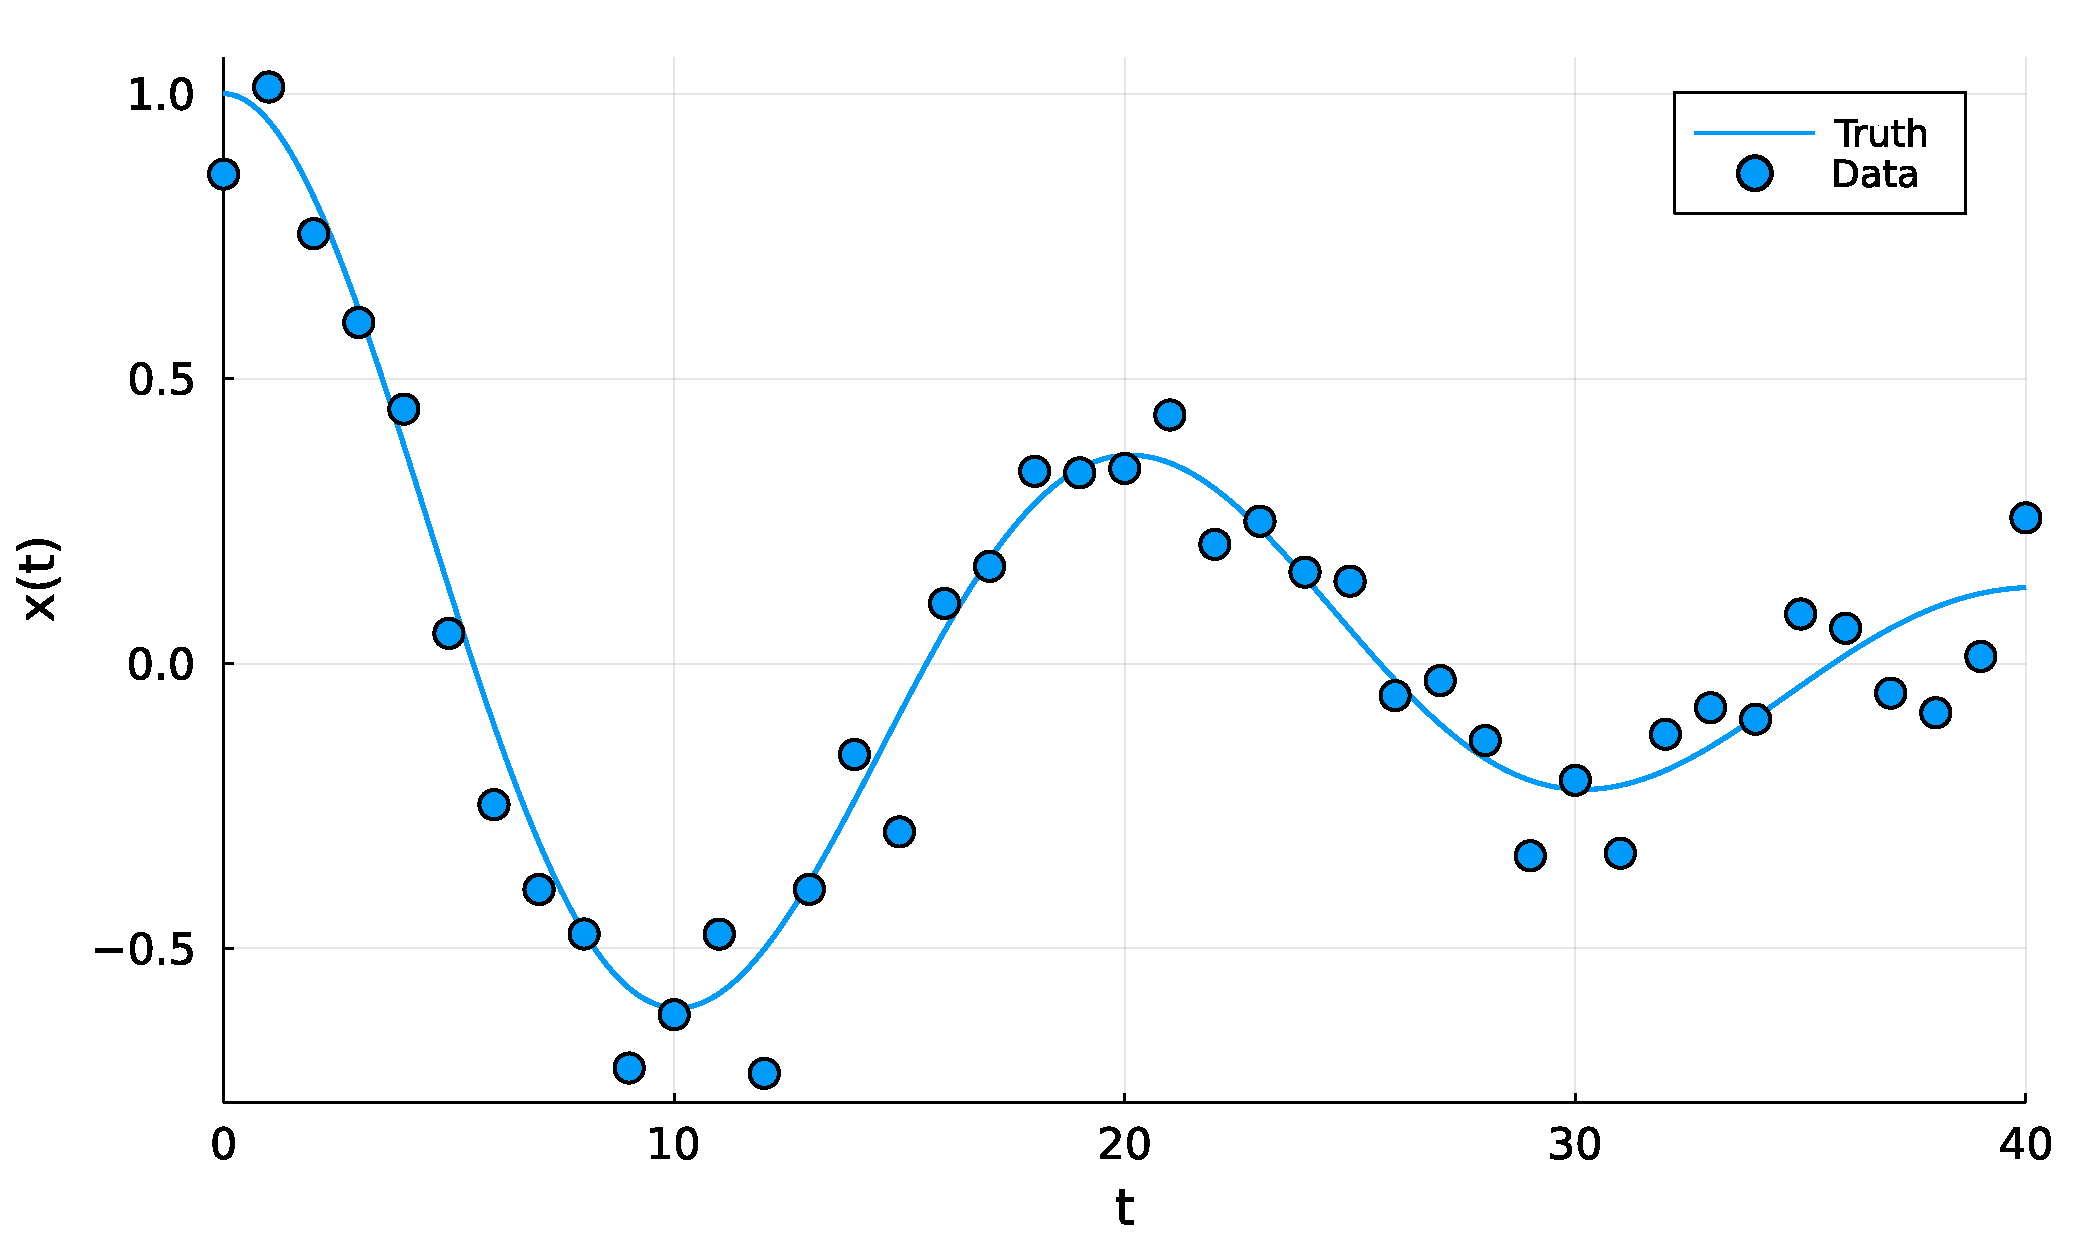
\includegraphics[width=\linewidth]{truth.pdf}
    \caption{The ODE solution is shown as the solid, blue line, and the simulated measurement data is shown as blue points.}
    \label{fig:DHO}
\end{figure}

I generate data from the ODE solution by taking equidistant time steps between $0$ and $40$ such that $\Delta t = 1.0$.
On top of this, I add some noise to the data to simulate measurement noise.
The blue points in Figure \ref{fig:DHO} are the data (including noise).

% \clearpage
\section*{2a: Naive Neural Network}

Now, having generated data, I try to fit the data directly with a neural network (NN).
That means, that I simply try to fit a neural network to the data without any prior knowledge about the model.
The neural network architecture is a classical neural network consisting of three dense layers:
${\mathbb{R} \rightarrow \mathbb{R}^{64} \rightarrow \mathbb{R}}$, or, as written in Julia:
\mbox{\texttt{Chain(x -> [x], Dense(1, 64, tanh), Dense(64, 1), first)}}.

With random initialization, the initial MSE loss is $26.2623$. After training (with \texttt{Optimization.jl}), it reduces to $0.0679$.
This seems to be working great, and apparently the neural network has learned how to fit the data quite well.
However, if one plots the (naive) neural network solution, it is clear that it has overfit the data, see Figure \ref{fig:NN_naive}.
This is even more apparent in the animations, see the attached file, \path{animation_NN_no_ode.gif}.

\begin{figure}[H]
    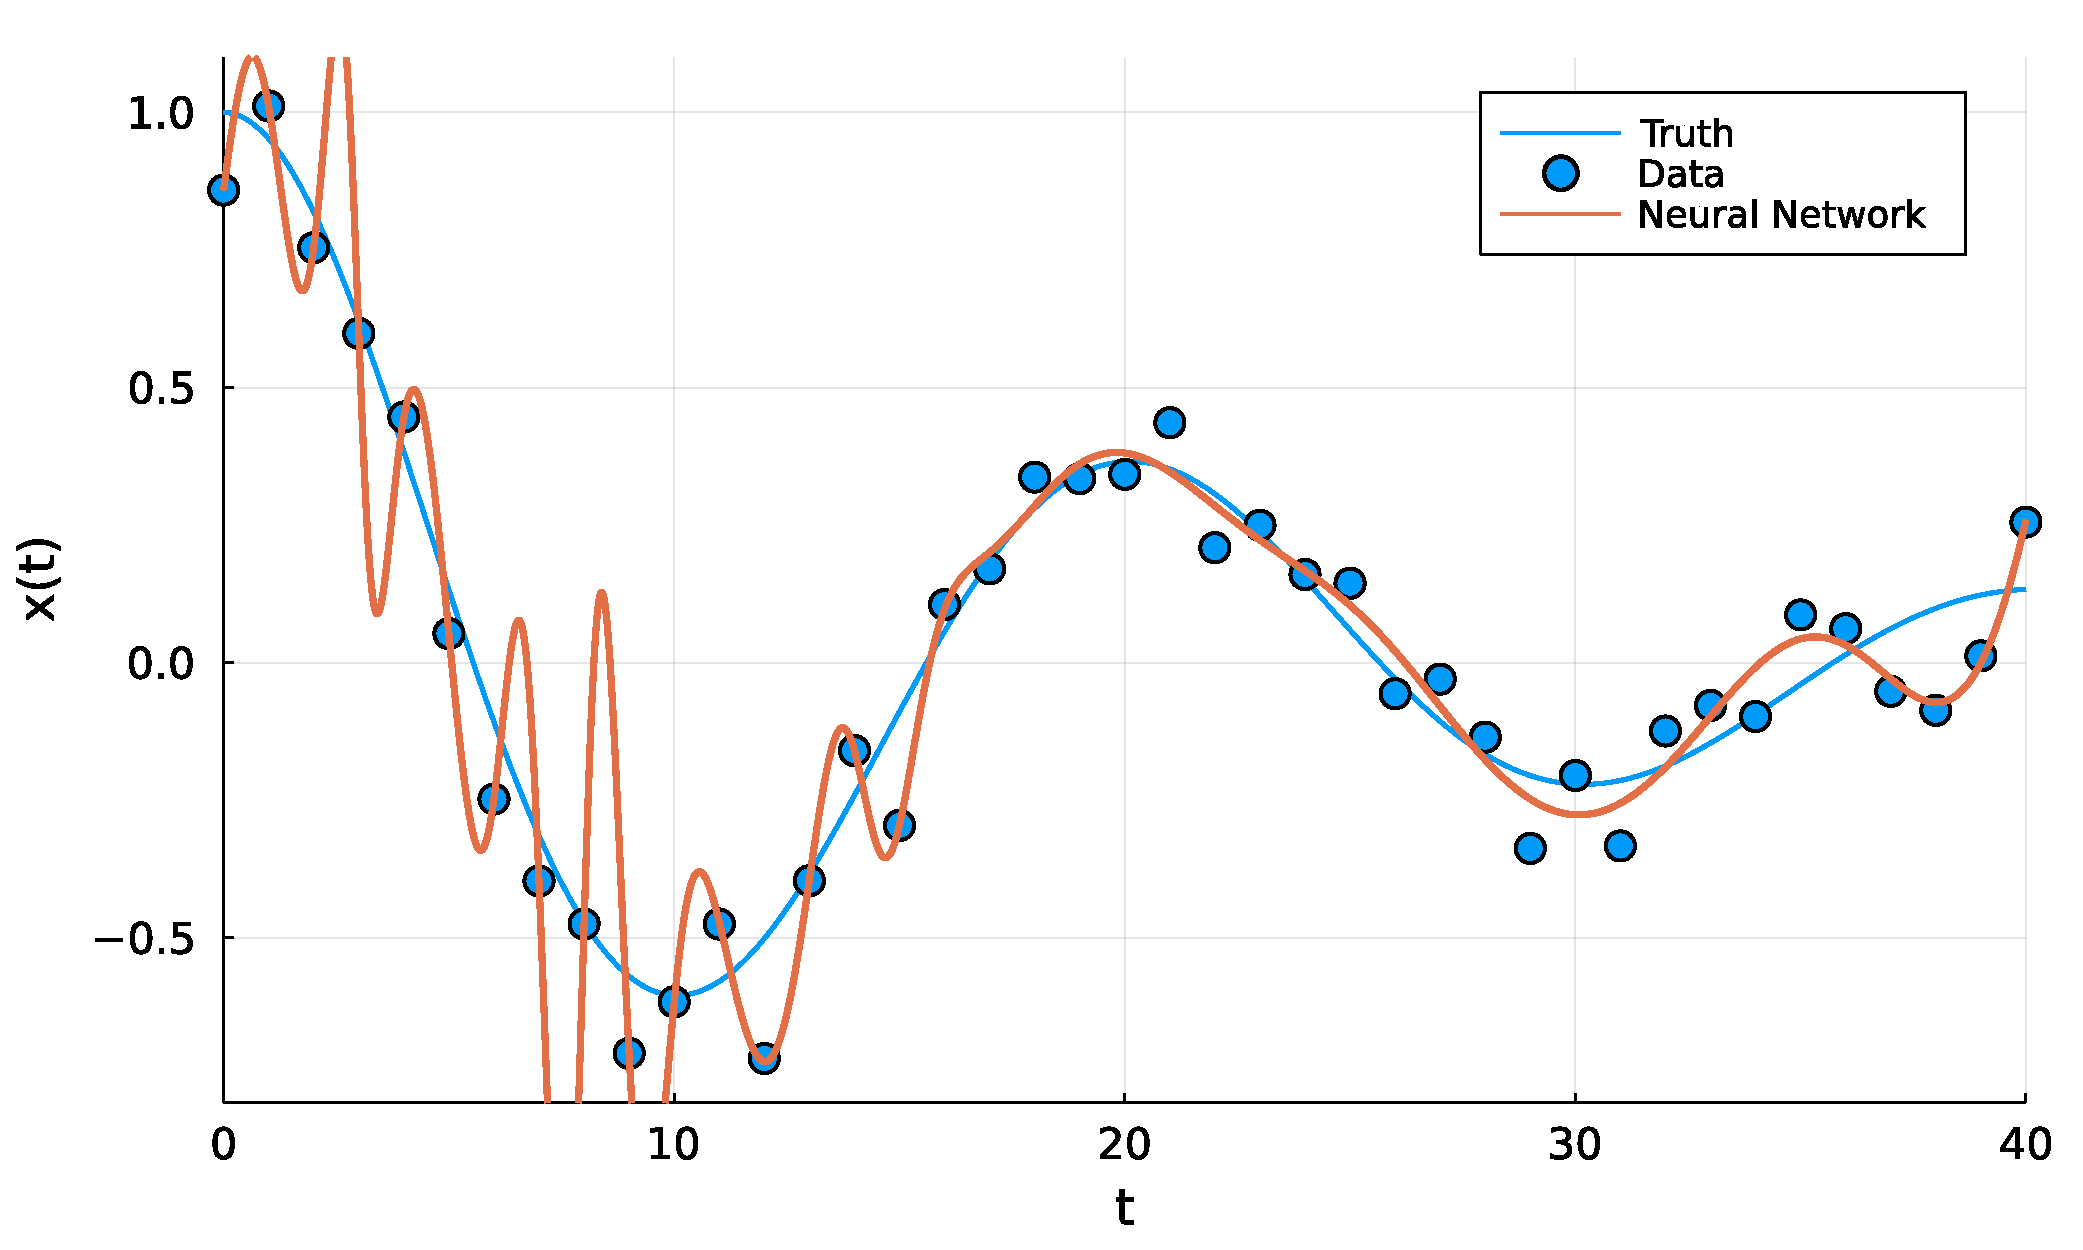
\includegraphics[width=\linewidth]{no_ode.pdf}
    \caption{The ODE solution is shown as the solid, blue line,
        the simulated measurement data is shown as blue points,
        and the naive neural network solution is shown as the solid, red line.}
    \label{fig:NN_naive}
\end{figure}

Another issue with this naive approach, is that the neural network solutions extrapolates very poorly.
Compare the extrapolation of the neural network to the true solution, see Figure \ref{fig:NN_naive_extrapolation}.
The solution oscillates around zero and asymptotically approaches it.
Yet, the neural network solution increases rapidly away from the true solution -- it has lost all predictive power.

\begin{figure}[H]
    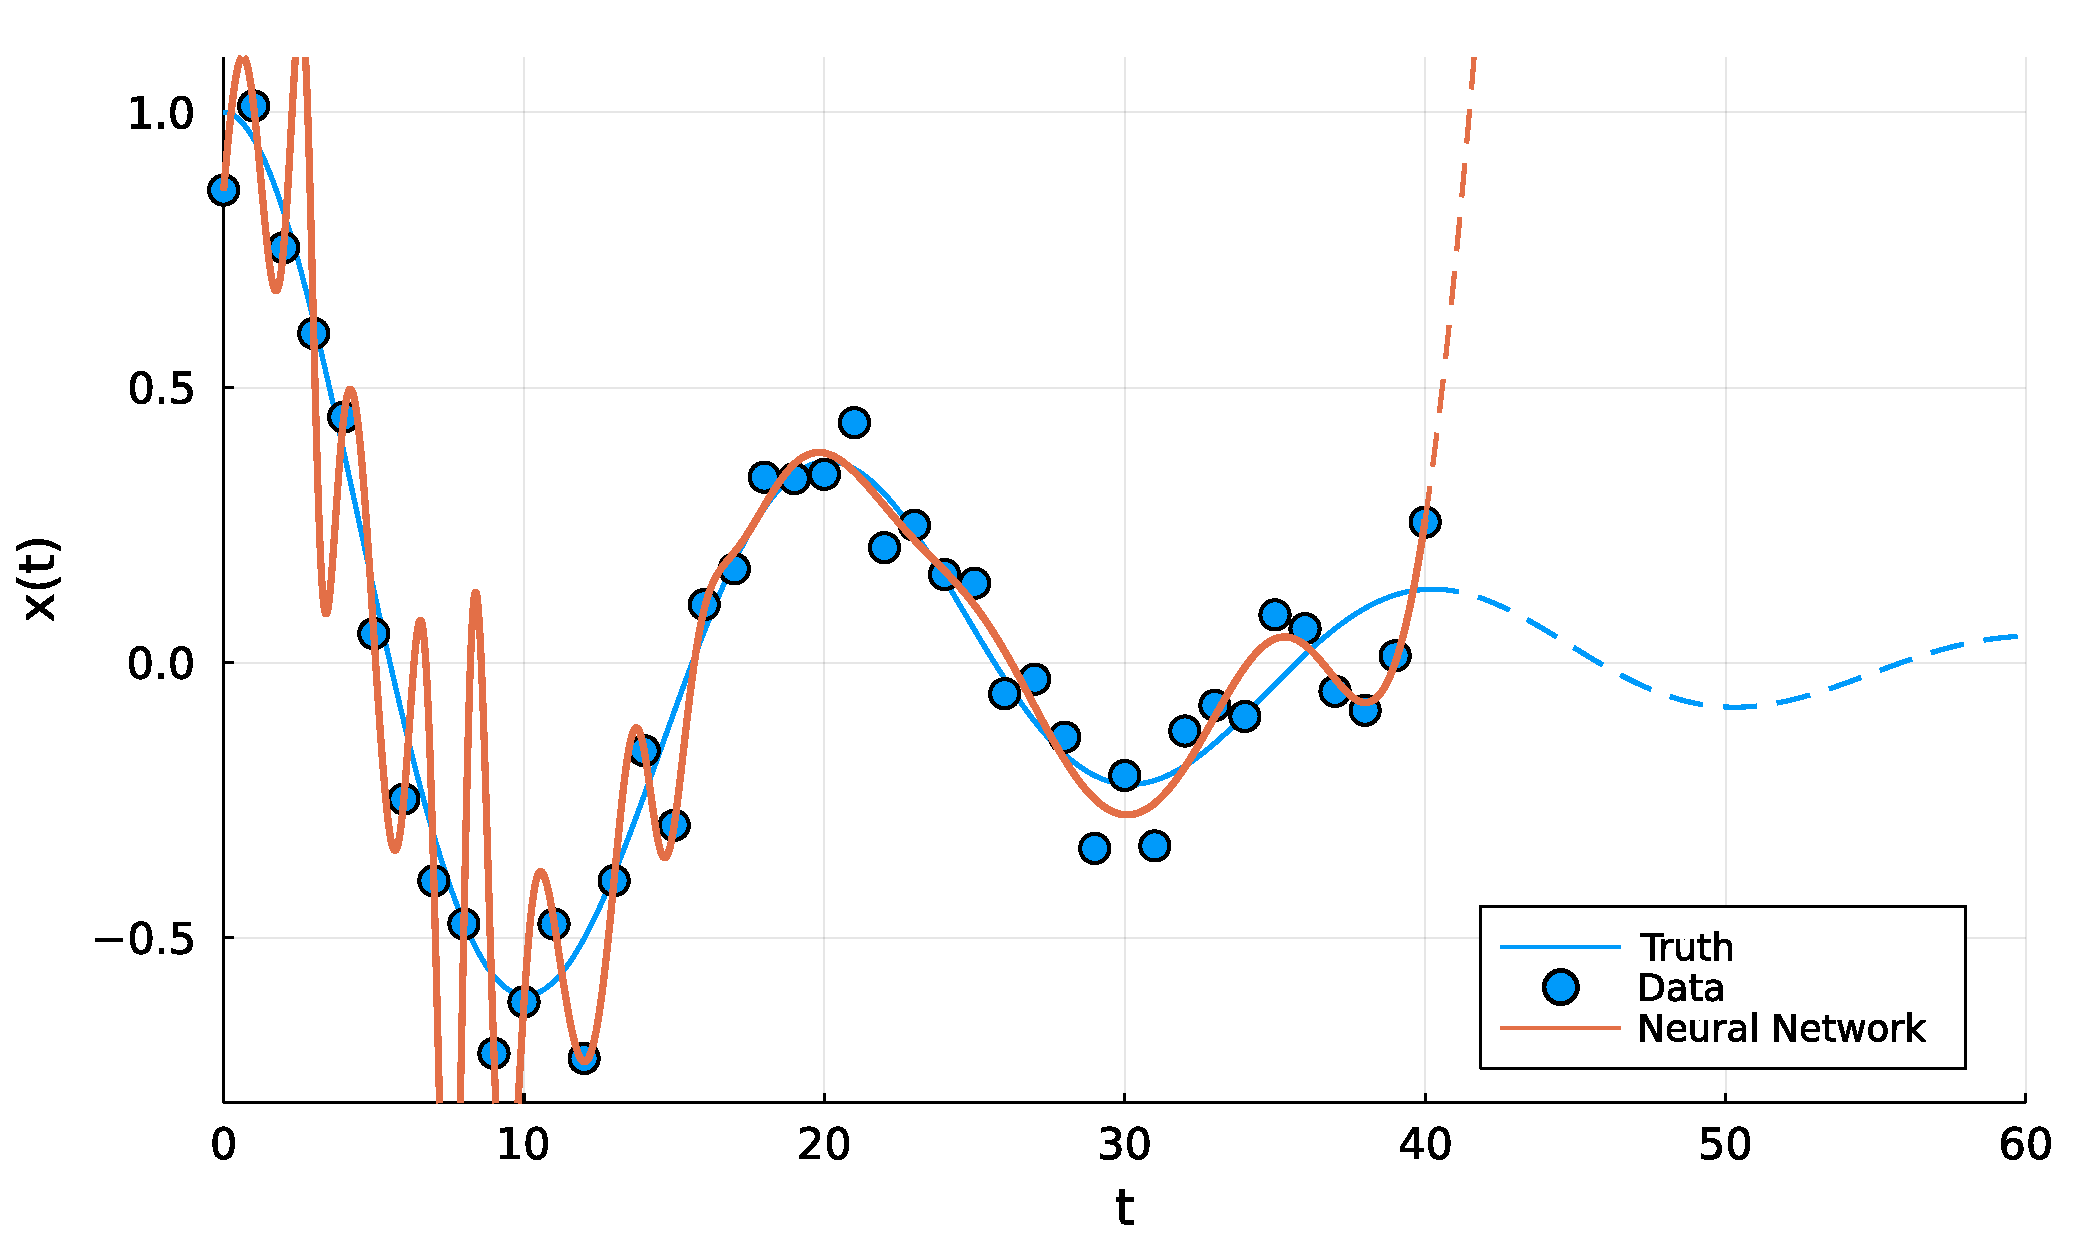
\includegraphics[width=\linewidth]{no_ode_etxrapolated.pdf}
    \caption{The ODE solution is shown as the solid, blue line,
        the simulated measurement data is shown as blue points,
        and the neural network solution is shown as the solid, red line.
        Extrapolations of the true solution and the neural network solutions are showed as dashed lines.}
    \label{fig:NN_naive_extrapolation}
\end{figure}

\section*{2b: Neural ODE}

Instead if fitting the neural network directly to the data, I combine it with some prior knowledge about the model.
In this case, I assume that I already know Newton's second law and Hook's law.
As such, it is only the friction term that is missing and what I want the neural network to learn.
Using the same form as in \eqref{eq:DHO_2D}, I can write this as:
\begin{equation}
    \begin{split}
        \dot{x} &= v \\
        \dot{v} &= -kx - \mathrm{NN}_\theta(v),
    \end{split}
    \label{eq:DHO_2D_NN}
\end{equation}
where $\mathrm{NN}_\theta(v)$ is the neural network with parameters $\theta$.
Here I have further incorporated the knowledge that the friction does not depend on position, but only velocity.
Note that I use a similar same neural network as the one in section 2a.

I now optimize the parameters of the neural network (and $k$), which reduces from a MSE loss of $583.8743$ to $0.3275$.
Even though the loss is higher than for the naive neural network, the solution is a lot better, see Figure \ref{fig:NN_ODE}.
This is even more apparent in the animations, see the attached file, \path{animation_NN_with_ode.gif}.

\begin{figure}[H]
    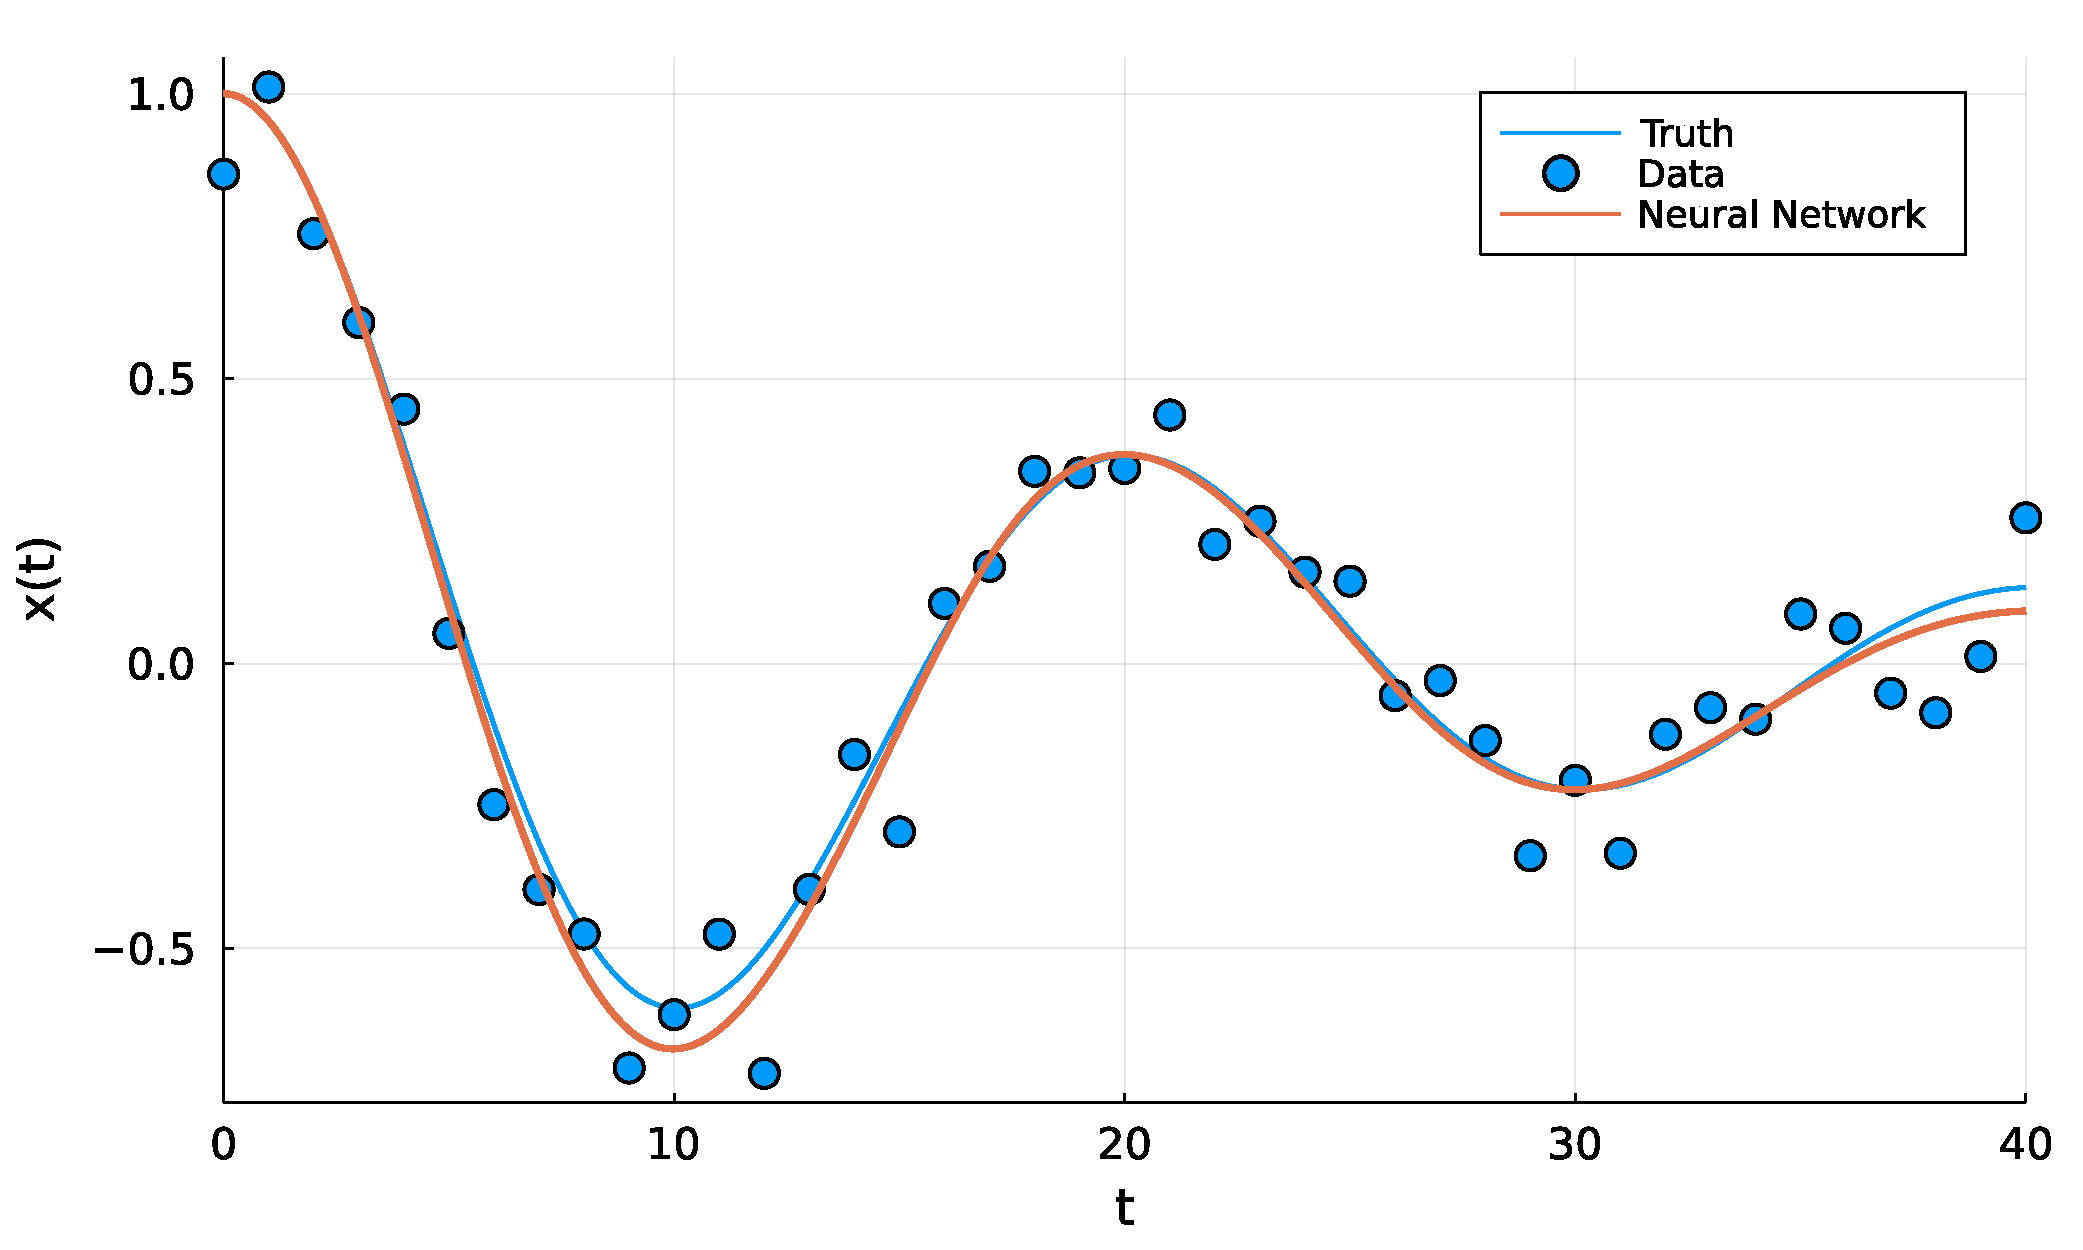
\includegraphics[width=\linewidth]{with_ode.pdf}
    \caption{The ODE solution is shown as the solid, blue line,
        the simulated measurement data is shown as blue points,
        and the neural ODE solution is shown as the solid, red line.}
    \label{fig:NN_ODE}
\end{figure}

Not only does this model not overfit, it also extrapolates a lot better, see Figure \ref{fig:NN_ODE_extrapolation}.
Compare this to Figure \ref{fig:NN_naive_extrapolation} which quickly diverged from the true solution.

\begin{figure}[H]
    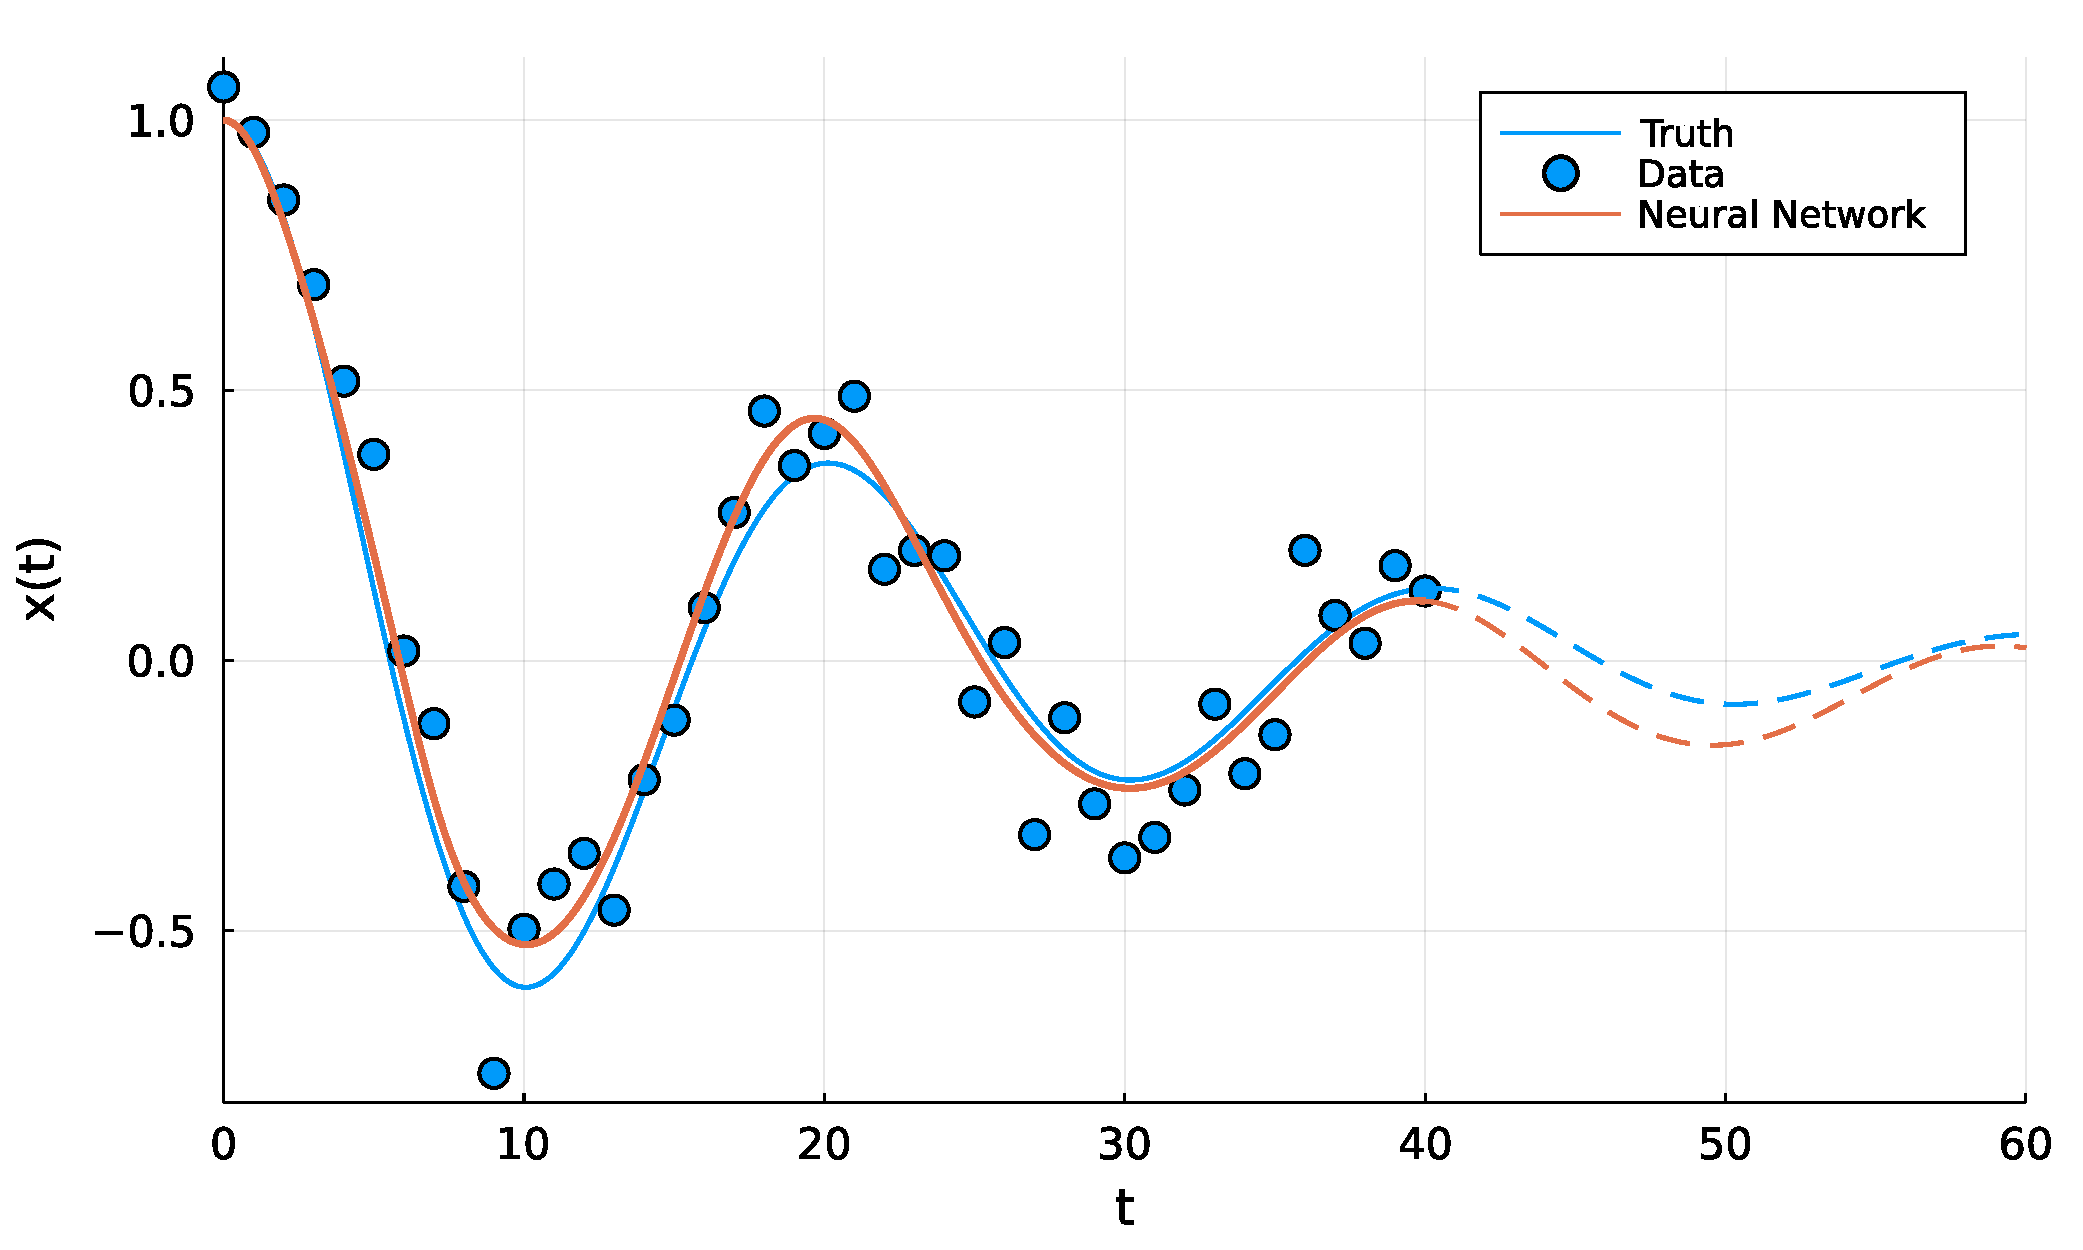
\includegraphics[width=\linewidth]{with_ode_extrapolated.pdf}
    \caption{The ODE solution is shown as the solid, blue line,
        the simulated measurement data is shown as blue points,
        and the neural ODE solution is shown as the solid, red line.
        Extrapolations of the true solution and the neural network solutions are showed as dashed lines.}
    \label{fig:NN_ODE_extrapolation}
\end{figure}

To further understand the neural ODE, I can also compare the true solution to the
neural ODE solution in the phase space. This is, instead of showing the solution
as a function of time, I show $x(t)$ on one axis and $v(t)$ on the other,
see Figure \ref{fig:NN_ODE_phase_space}.
Here I note some discrepencies between the true solution and the neural ODE solution,
however, the neural ODE solution seems to capture the overall shape of the true solution.

\begin{figure}[H]
    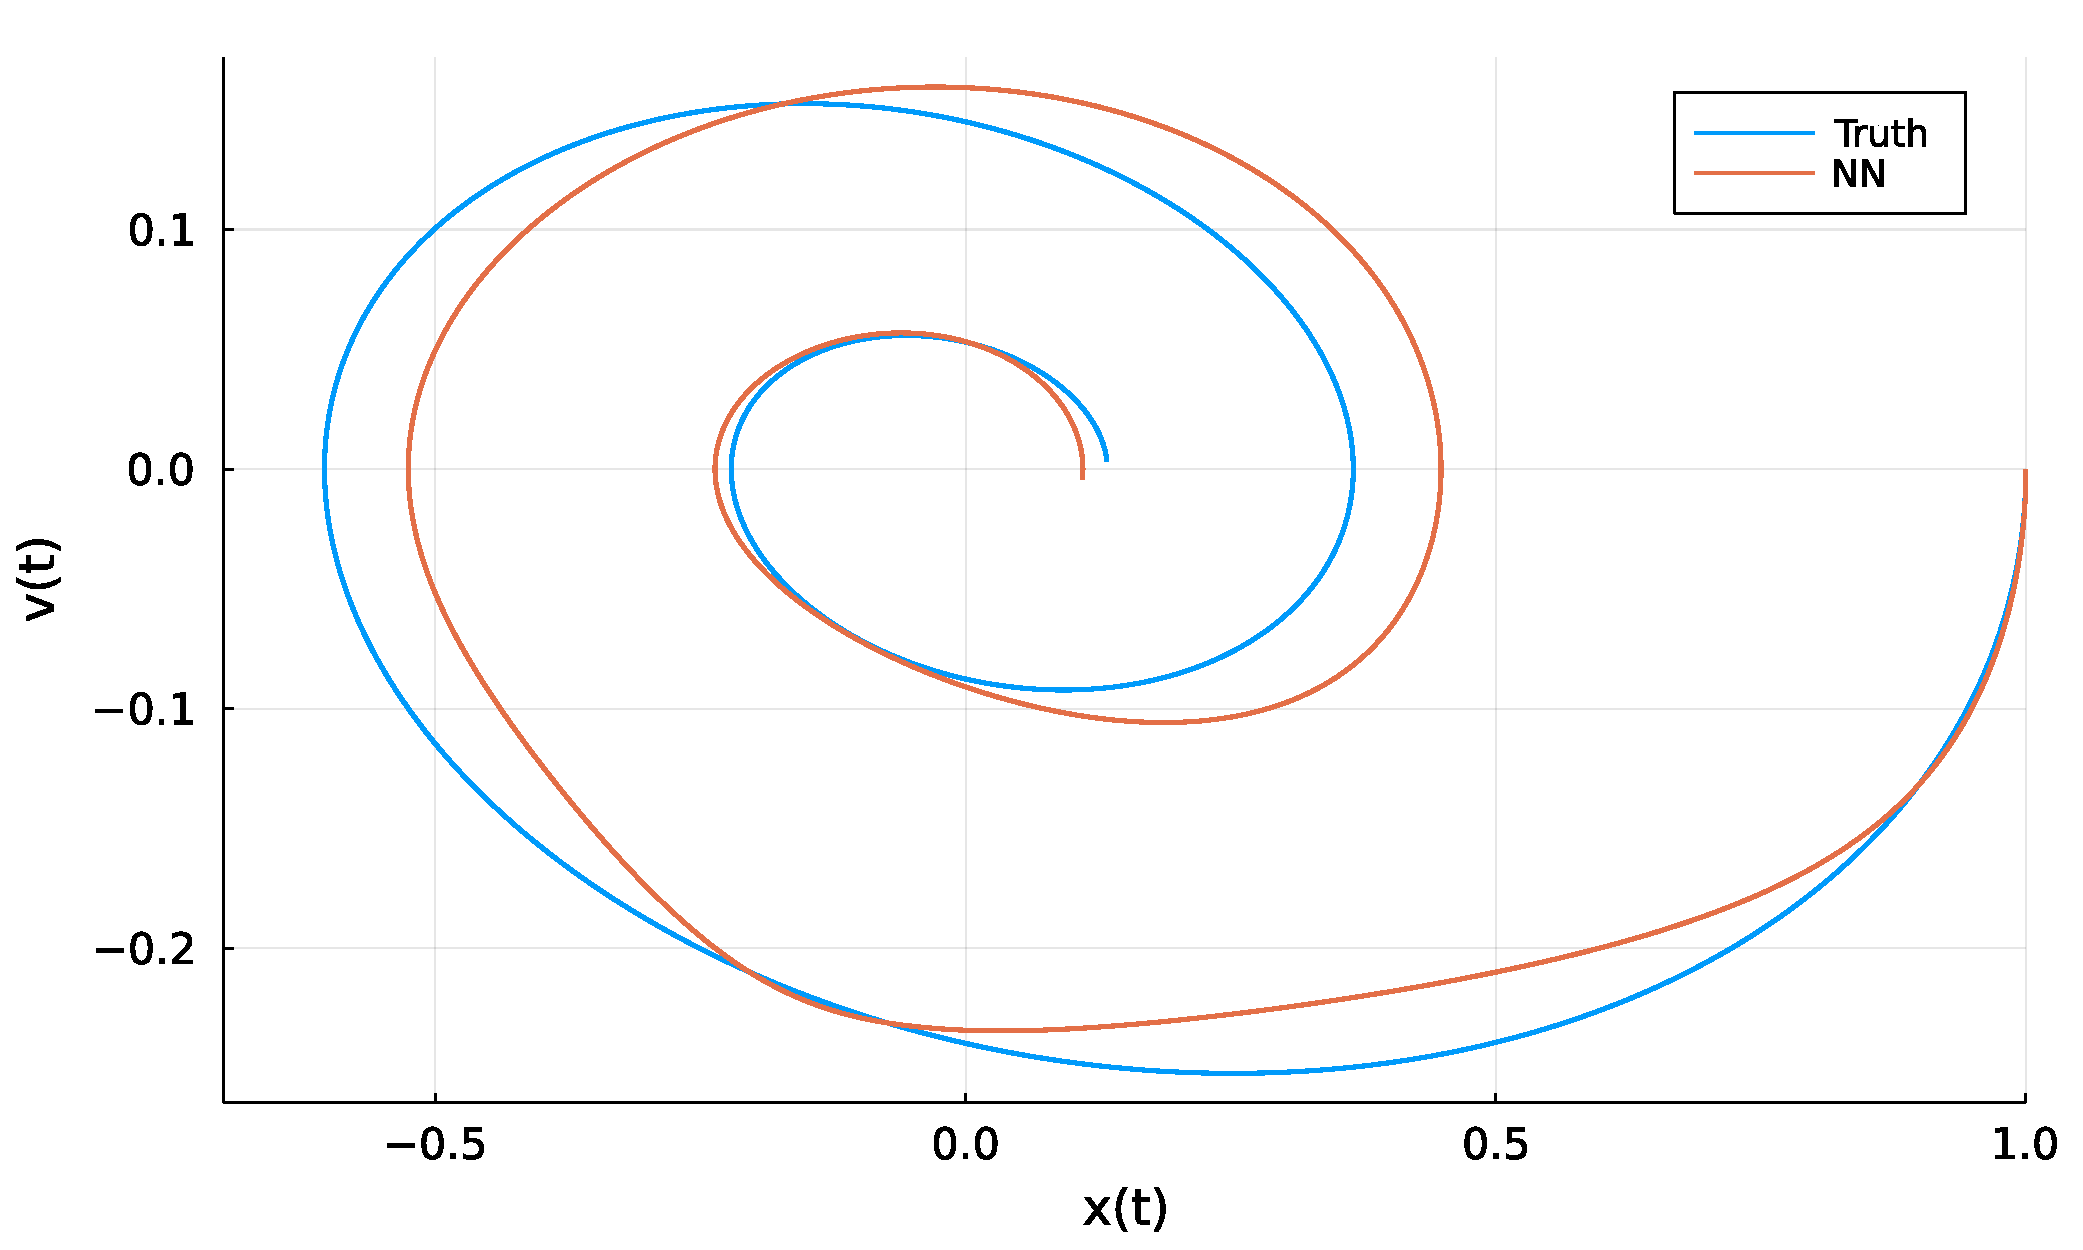
\includegraphics[width=\linewidth]{phase_space.pdf}
    \caption{The ODE solution is shown as the solid, blue line,
        and the neural ODE solution is shown as the solid, red line.}
    \label{fig:NN_ODE_phase_space}
\end{figure}


\section*{3: Symbolic Regression}

Before I do any symbolic regression on the neural network, I first try to visualize it, see Figure \ref{fig:NN}.
At first, it does not seem like any ``textbook'' function, however, if I only look at the
interval from $-0.3 < v < 0.15$, which is the range of values of $v$ that the neural network was actually trained on,
see the y-axis of Figure \ref{fig:NN_ODE_phase_space}, I notice that it is (surprisingly) linear.

\begin{figure}[H]
    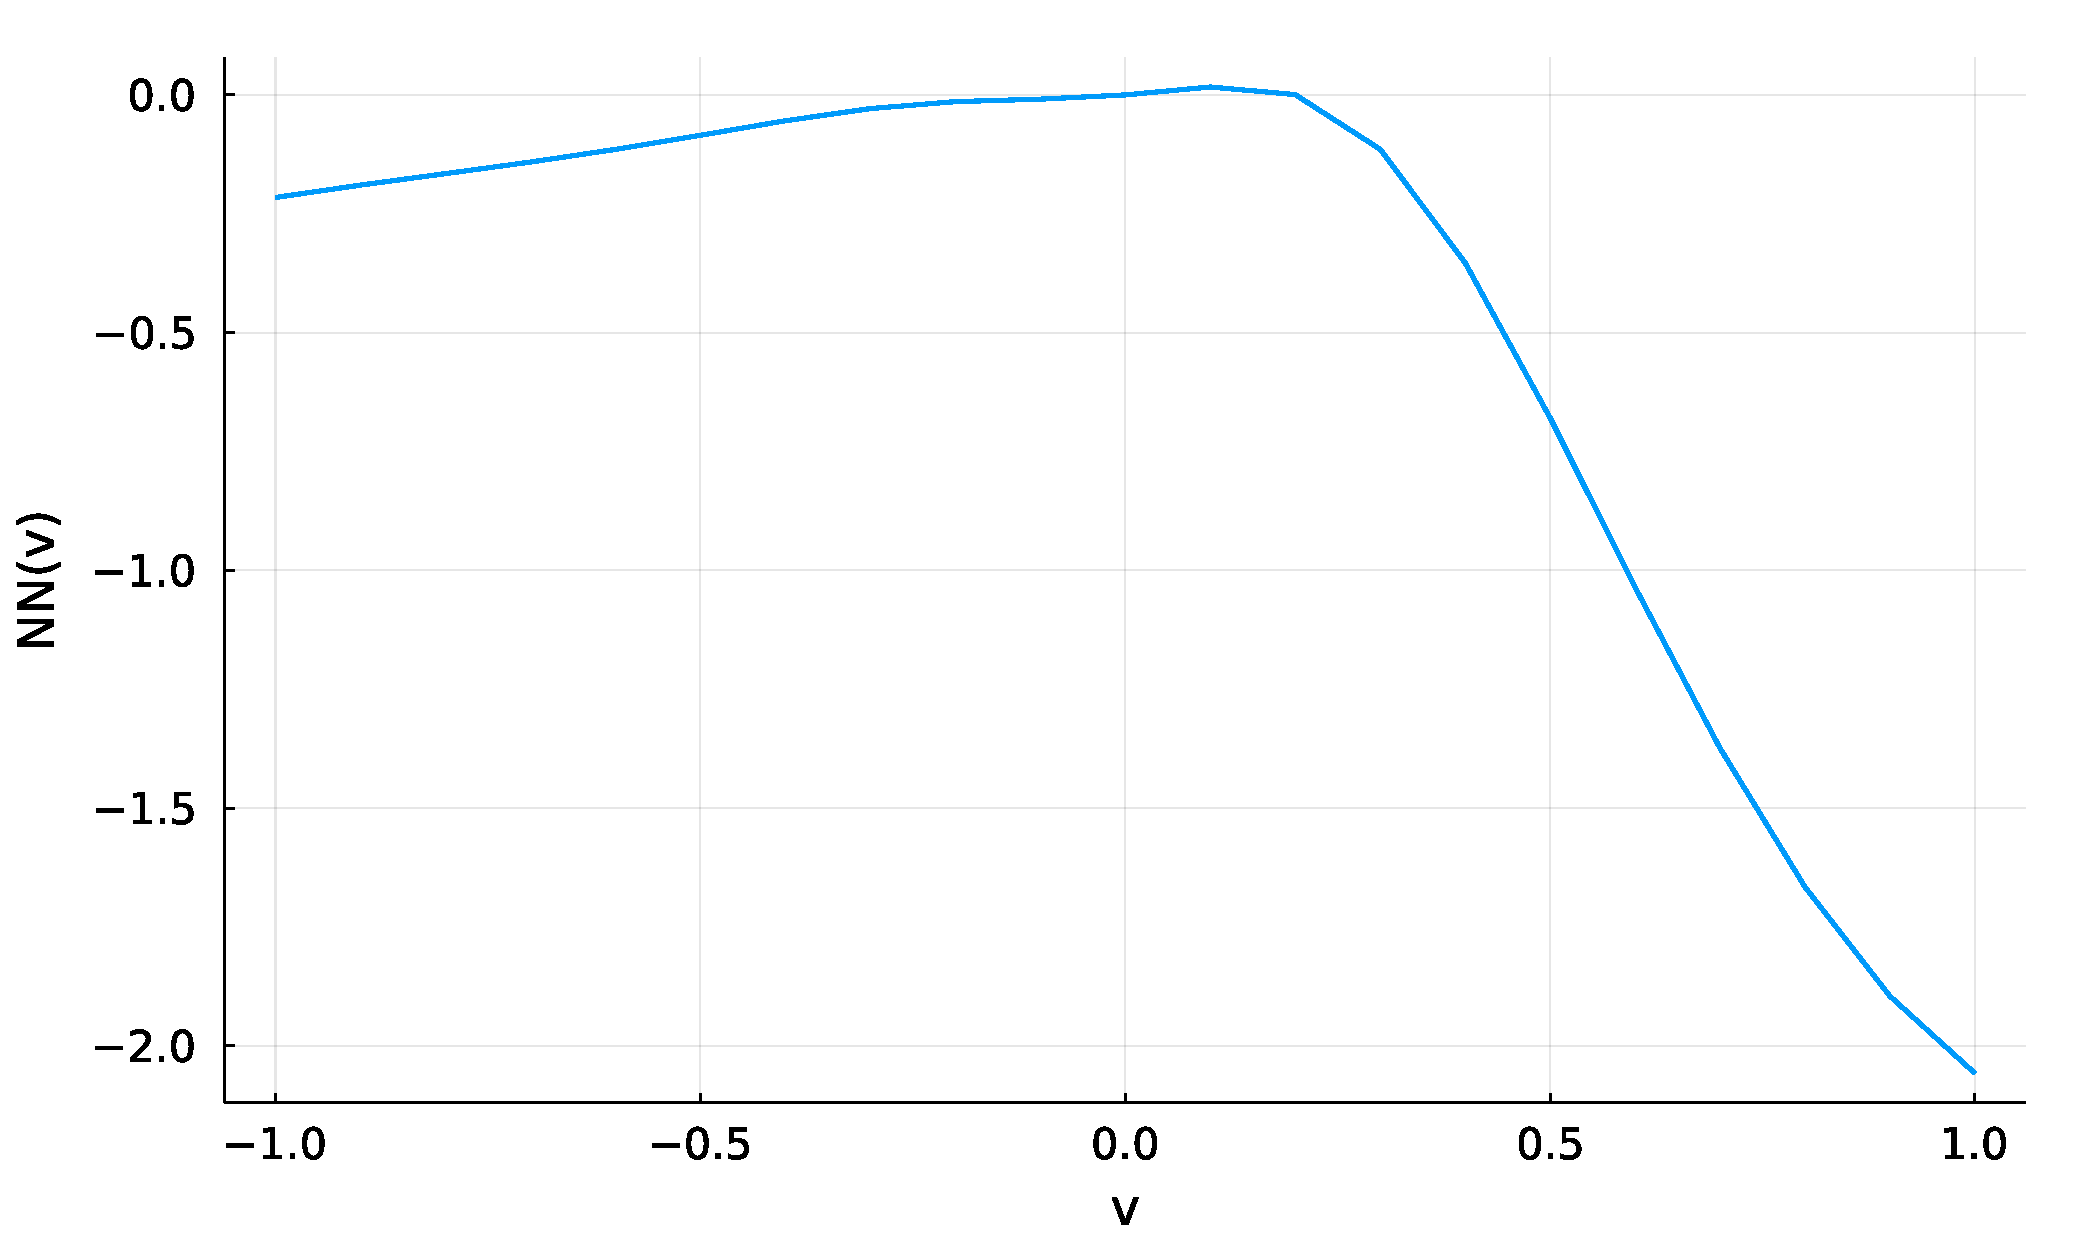
\includegraphics[width=\linewidth]{nn.pdf}
    \caption{The output of the neural network as a function of velocity, $v$.}
    \label{fig:NN}
\end{figure}

I perform the symbolic regression on the neural network using \texttt{DataDrivenDiffEq.jl}
where I use the \texttt{DirectDataDrivenProblem} function in particular.
I use $u[1]$ and $u[2]$ as variables and set up a basis consisting of
$\sin(u[1])$, $\sin(u[2])$, $\cos(u[1])$, $\cos(u[2])$ along with
polynomial basis functions up to order 5: in total 25 elements.
I use the \texttt{ADMM} optimizer to introduce sparseness in the solutions (via Lasso).
I find that the problem found a solution with a loss of $L_2$ Norm error of $0.002496$.
The solution was:
\begin{verbatim}
    Model ##Basis#638 with 1 equations
    States : u[1] u[2]
    Parameters : p₁
    Independent variable: t
    Equations
    φ₁ = p₁*u[2]
\end{verbatim}

The symbolic regression was able to retrieve the correct function form of the
missing part of the ODE and correctly found that the solution only depends on
$u[2]$ i.e. the velocity and not on $u[1]$, the position:

\begin{equation}
    \mathrm{NN}_\theta \approx b * v
\end{equation}

\section*{4: Bayesian Inference}

Now that I know the functional form of the ODE, I can use the Bayesian inference
to estimate the value of the unknown parameters, $b$ and $k$, using \texttt{Turing.jl}.

I assume that $b$ is a random variable drawn from a normal distribution (truncated to be positive)
and similar for $k$. I first compute the MAP estimate to initialize the MCMC chains at this point.
I then run 4 chains, each for 1000 iterations, using the NUTS sampler, see Figure \ref{fig:MCMC_chains}.
I also estimate the size of the noise, $\sigma$, which is also shown in this figure.
The noise is slightly overestimated, however both $b$ and $k$ matches the true values.

\begin{figure}[H]
    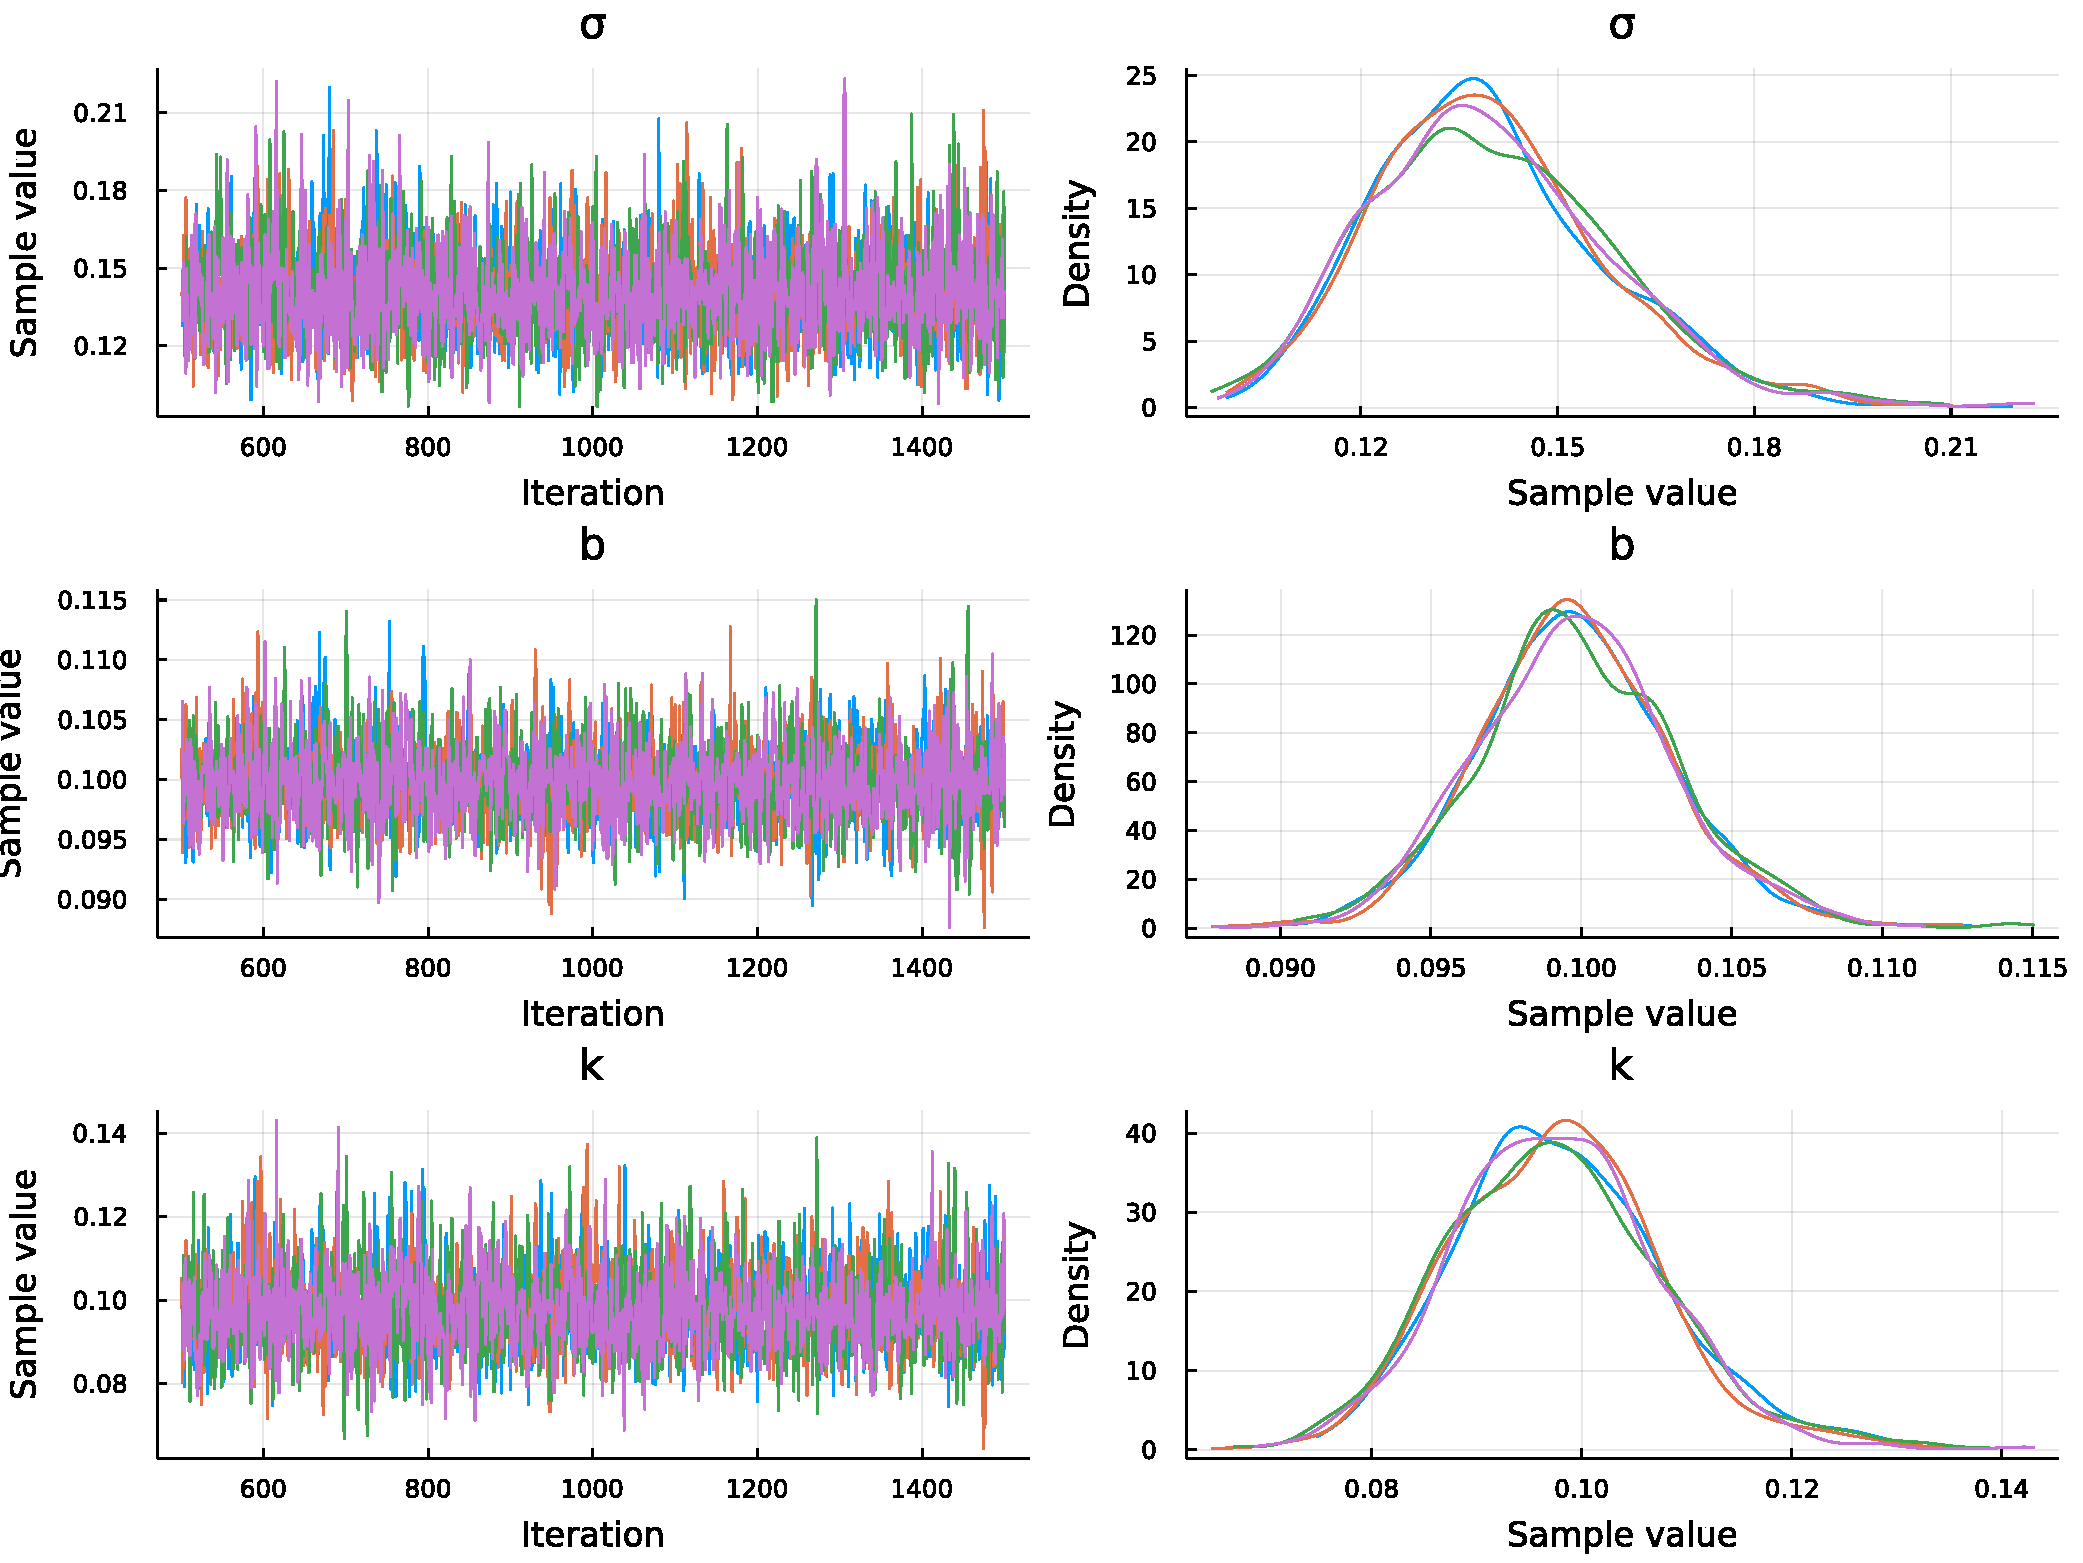
\includegraphics[width=\linewidth]{turing_chains.pdf}
    \caption{Left) The trace plots for the MCMC chains. Right) The density plots for the MCMC chains.}
    \label{fig:MCMC_chains}
\end{figure}

Having the posterior samples available in the MCMC chains, I also visualize how the
uncertainties on the parameters affect the ODE solution in Figure \ref{fig:MCMC}.
Note that the since I assumed the initial positions to be known without any
uncertainties, the $x(t)$ all start at the same value and then slowly increase in uncertainty
as a function of time.

\begin{figure}[H]
    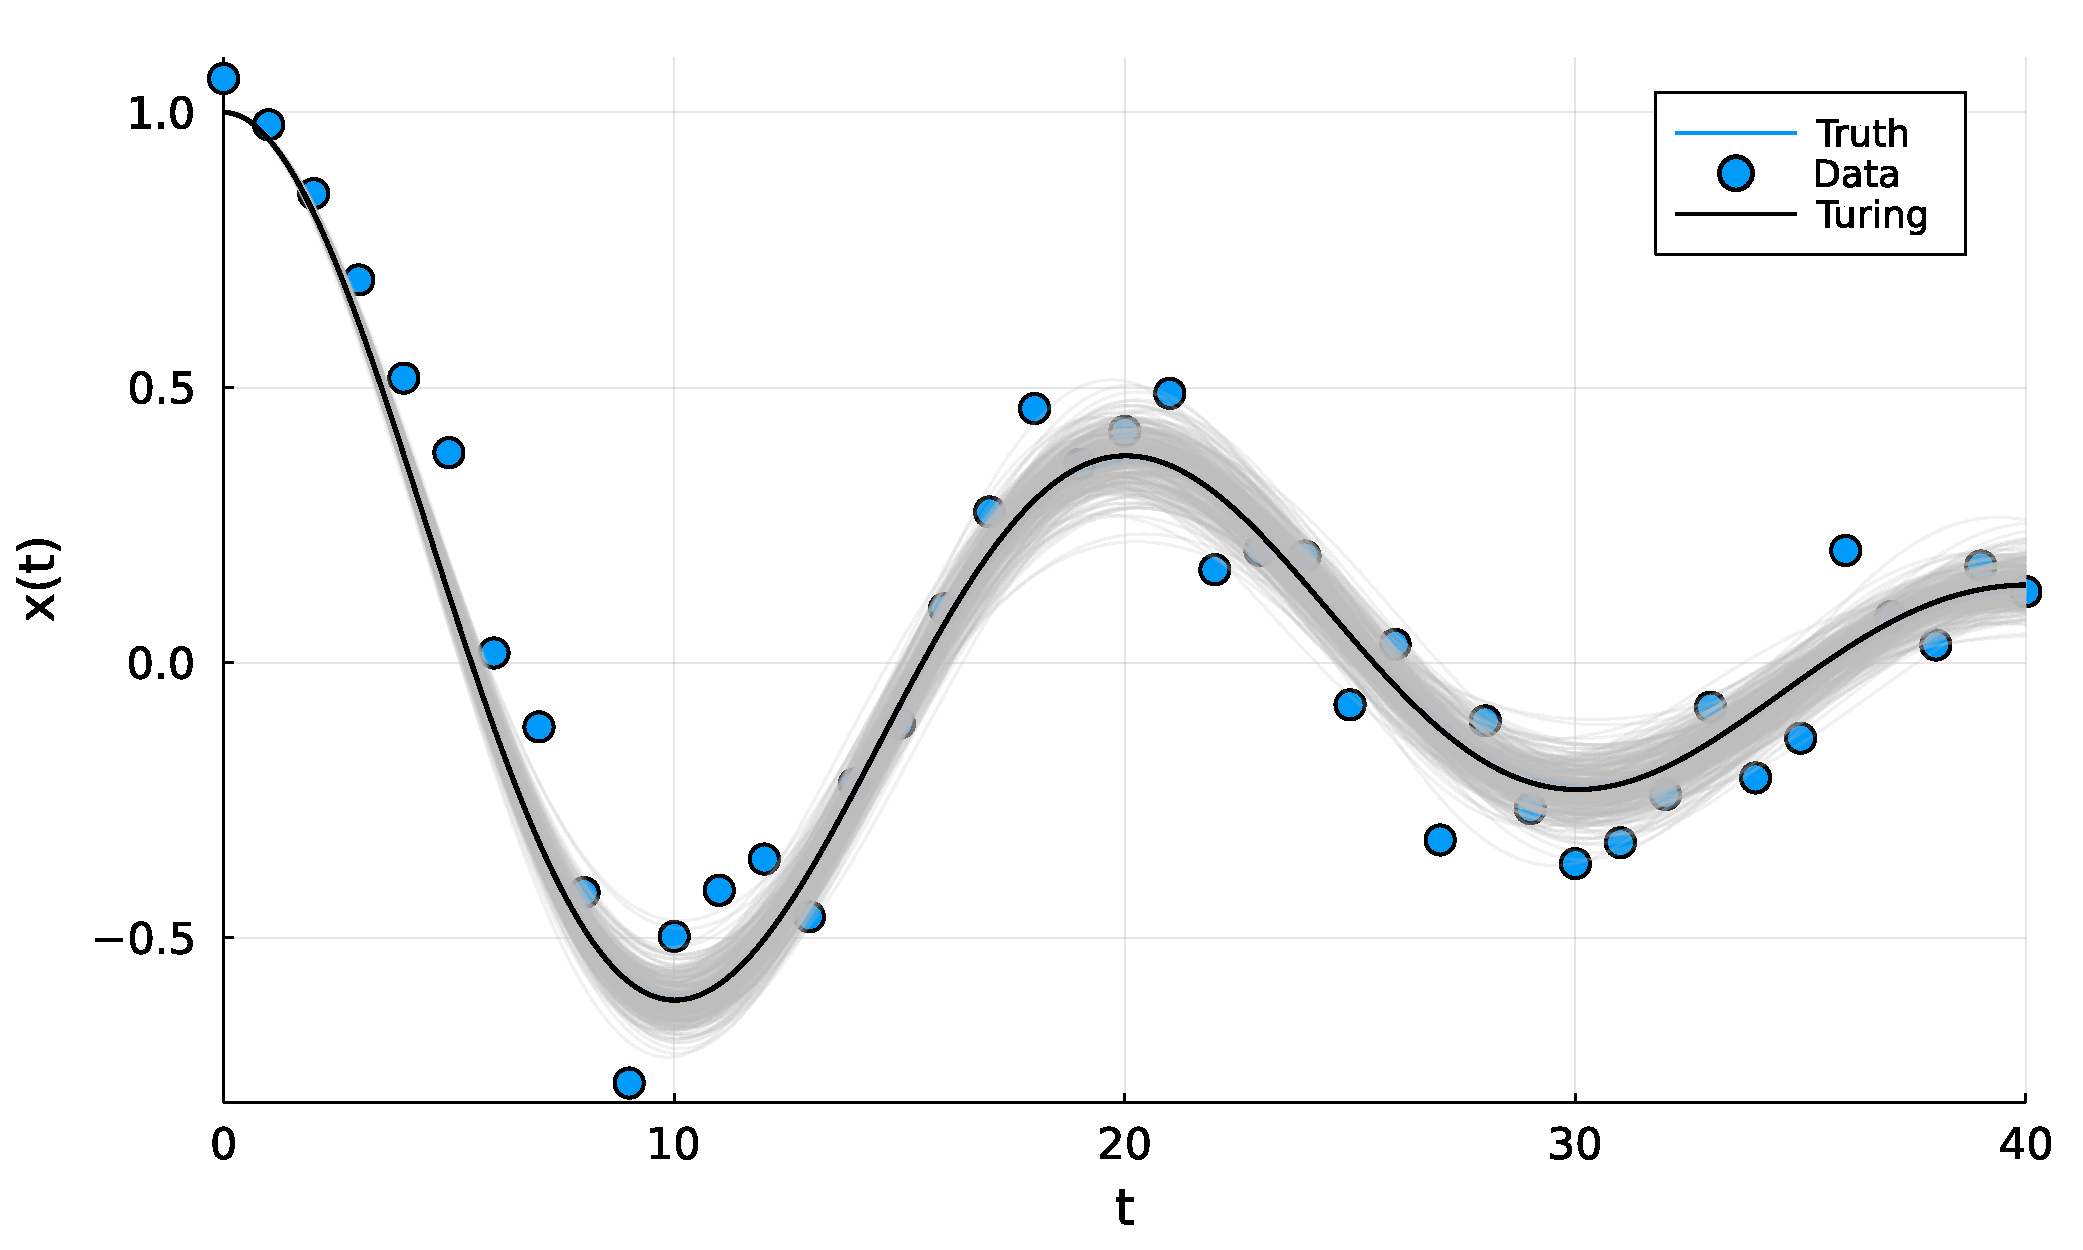
\includegraphics[width=\linewidth]{turing.pdf}
    \caption{The ODE solution is shown as the solid, blue line,
        the simulated measurement data is shown as blue points,
        and the ODE solutions of 300 traces from the posterior distribution are shown grey lines.}
    \label{fig:MCMC}
\end{figure}


\section*{Conclusion}
In this small project, I have shown how fitting a neural network in the phase space,
combined with prior knowledge, allows for better predictions compared to the naive approach.
In addition, it also generalizes significantly better and extrapolates quite well.

Using symbolic regresion, it is possible to retrieve the functional form of the
dynamics that the neural network has learned to predict and which was missing
from the ODE. Using this new functional form, it is possible to estimate the parameters using
Bayesian MCMC inference.


\end{document}